To validate the stability of the BDTs, the impact on final results when varying the BDT training was studied for each leptoquark mass hypothesis. This study was performed with 2016, 2017, and 2018 simulation. The BDTs used are from an early training performed on just 2016 simulation, with only preselection, b-jet tag requirements, MC corrections, and background normalization applied. Additionally, the DeepJet scores of the two leading jets were included as input variables to the trainings (these were dropped for the final analysis). For each leptoquark mass hypothesis, a cut on the score of the BDT trained with the neighboring leptoquark mass point (up or down) was applied. BDT score thresholds are taken from Table~\ref{tab:cutlog} (where \MLQ would represent leptoquark mass point in the BDT training). Asymptotic expected upper limits at  \SI{95}{\%} \CL were set for each leptoquark mass hypothesis using the varied BDTs. Figure~\ref{figapp:BDTstudy} shows the asymptotic expected upper limit on $\sigma(\HepProcess{\Pp\Pp \to \LQ\LQbar})$ as a function of the leptoquark mass hypothesis using the ``up'' and ``down'' varied BDTs. In the case where the BDT was trained at a leptoquark mass point below the leptoquark mass hypothesis, the lower bound placed on the leptoquark mass varied by year relative to the nominal bound. When the BDT was trained at a leptoquark mass point above the leptoquark mass hypothesis, the expected lower bound placed on the leptoquark mass was noticably lower, compared to the nominal bound. Table~\ref{tab:limitsBDTstudy} lists the expected lower bounds on the leptoquark mass derrived from this study for each year of data-taking. To observe BDT stability, the ratio of the expected limits (where the numerator is the ``up'' or ``down'' varied expected limit and the denominator is the nominal expected limit) is shown for 2016, 2017, and 2018 in Figure~\ref{figapp:BDTratio}.

\begin{table}[htbp]
    \caption{Expected lower bounds on the leptoquark mass placed using a BDT trained with a leptoquark mass point equal to, varied down from, and varied up from the leptoquark mass hypothesis in 2016, 2017, and 2018 simulation. In parentheses are the percent differences of the varied lower bounds from the nominal lower bound.}
    \begin{center}
           %\scriptsize
           \begin{tabular}{cccc}\hline\hline
                        & \multicolumn{3}{c}{Expected asymptotic limit (relative difference)} \\
                Year    & Nominal [GeV] & Varied down [GeV] (\%) & Varied up [GeV] (\%) \\ \hline
                2016    & 1591.2 & 1591.5 (0.02) & 1572.9 (1.2) \\
                2017    & 1597.3 & 1572.1 (1.6) & 1578.7 (1.2) \\
                2018    & 1641.6 & 1661.8 (1.2) & 1620.2 (1.3) \\ \hline\hline
           \end{tabular}
           \label{tab:limitsBDTstudy}
    \end{center}
\end{table}

\begin{figure}[htbp]
    \centering
    {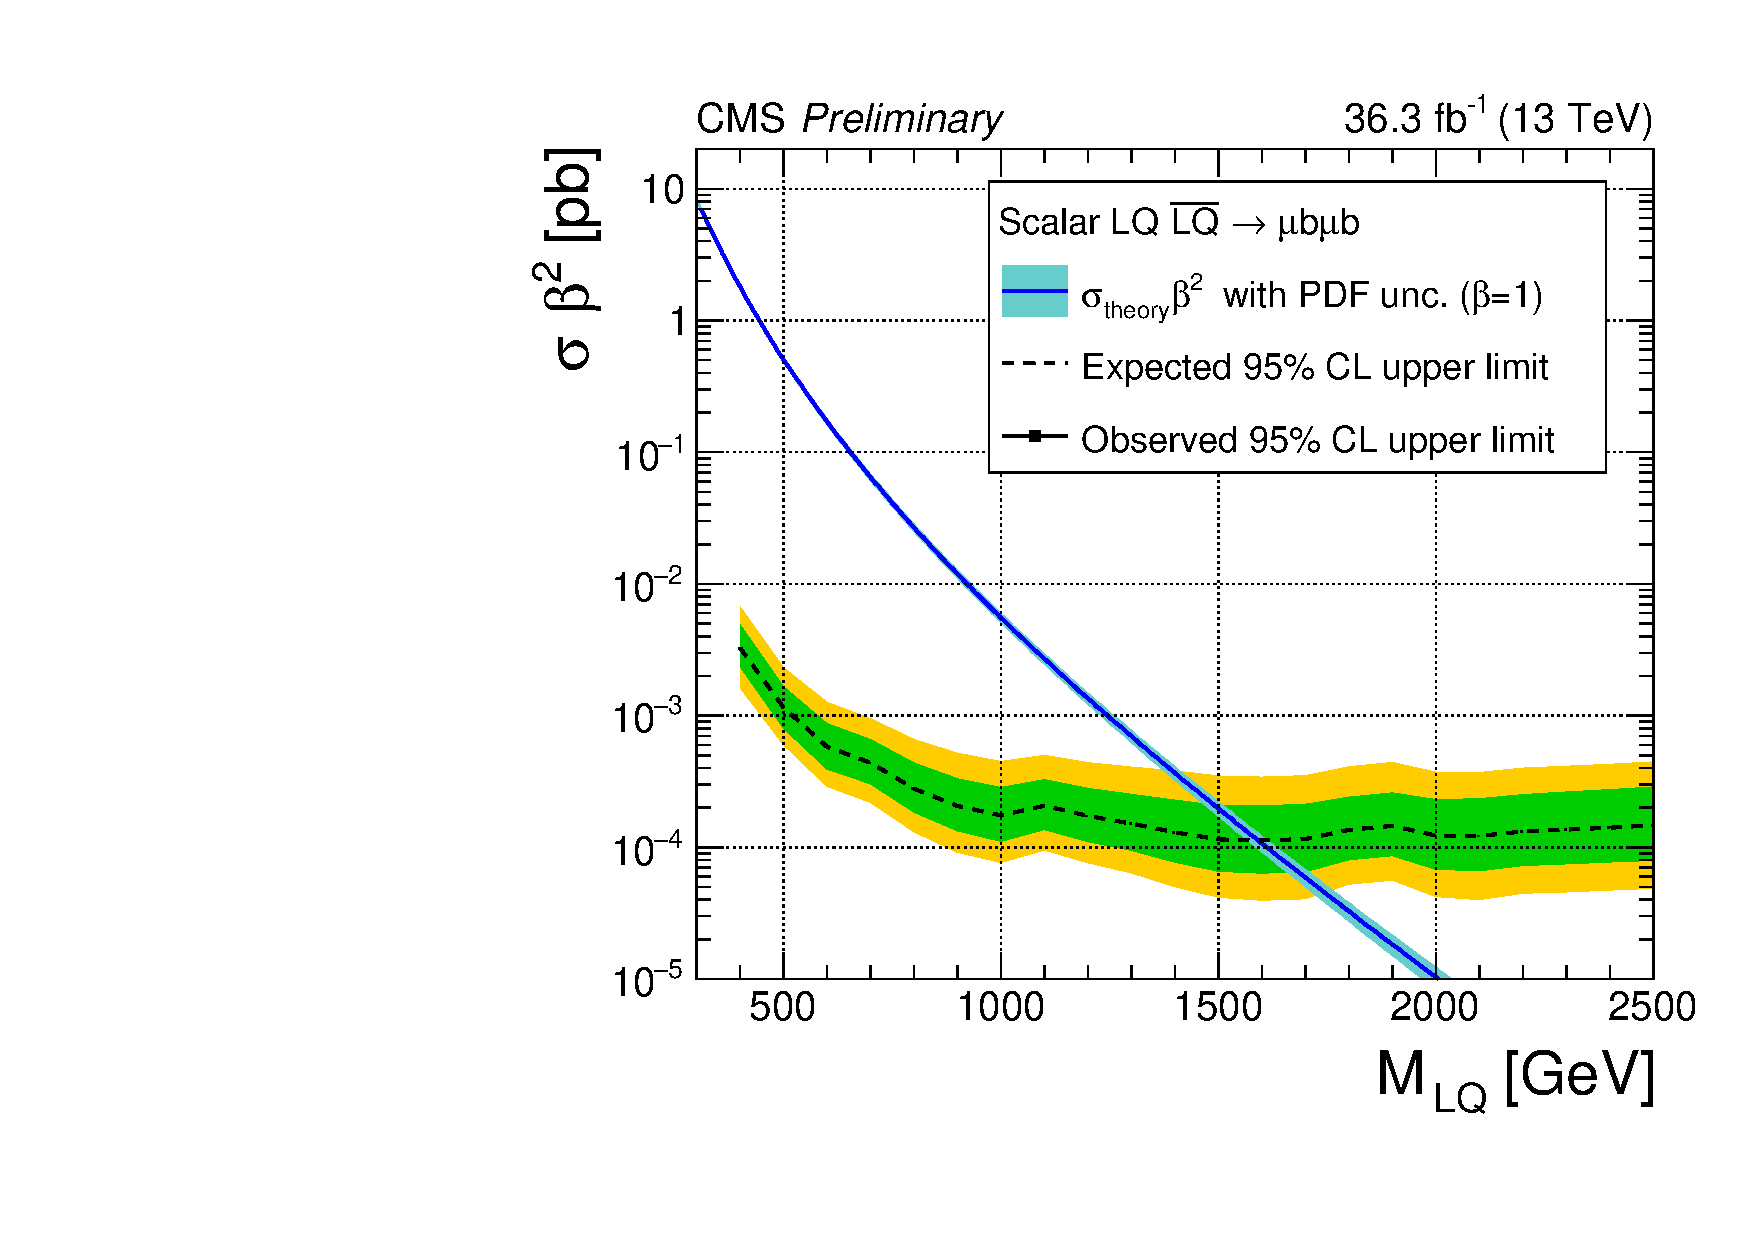
\includegraphics[width=.32\textwidth]{Images/Analysis/BDT_Study_plots/BR_Sigma_MuMu_2016_BDTStudy_Down.pdf}}
    {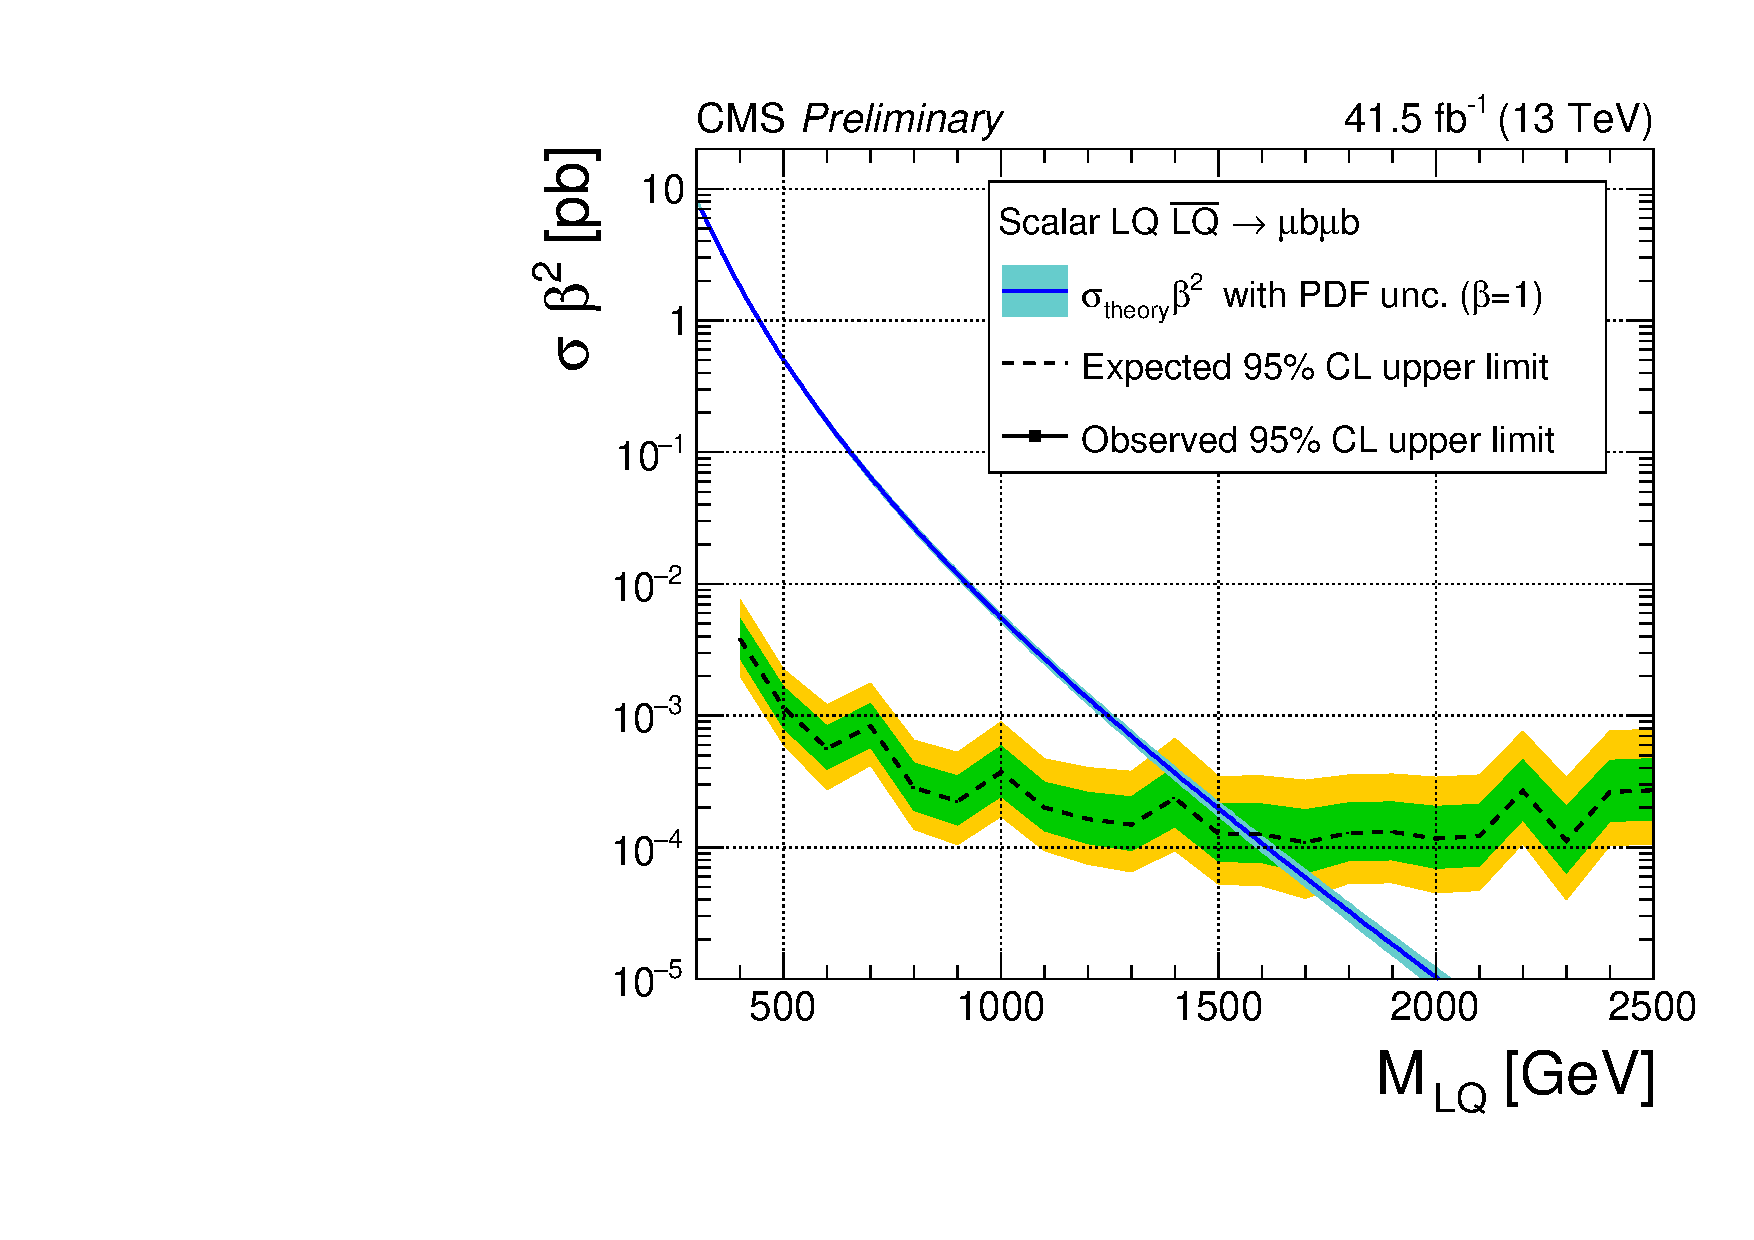
\includegraphics[width=.32\textwidth]{Images/Analysis/BDT_Study_plots/BR_Sigma_MuMu_2017_BDTStudy_Down.pdf}}
    {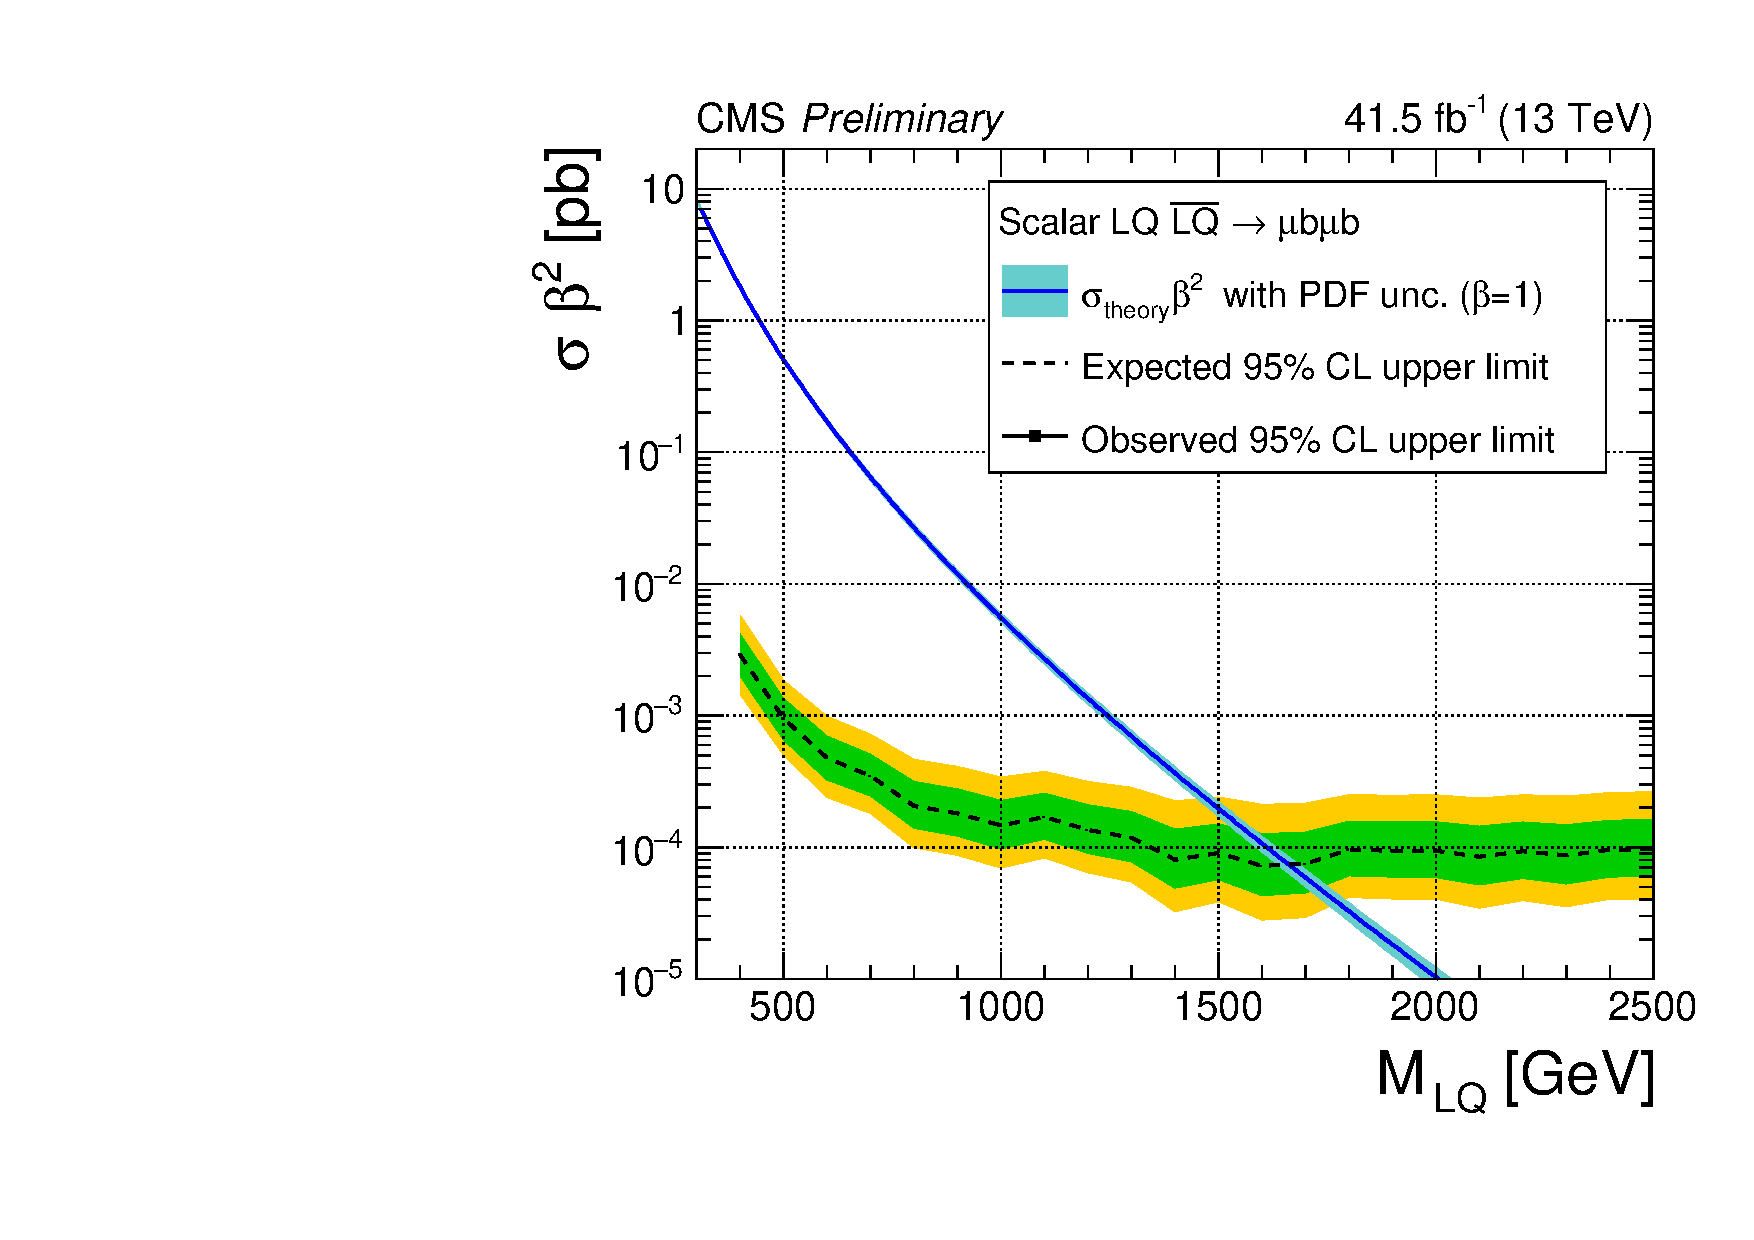
\includegraphics[width=.32\textwidth]{Images/Analysis/BDT_Study_plots/BR_Sigma_MuMu_2018_BDTStudy_Down.pdf}}
    {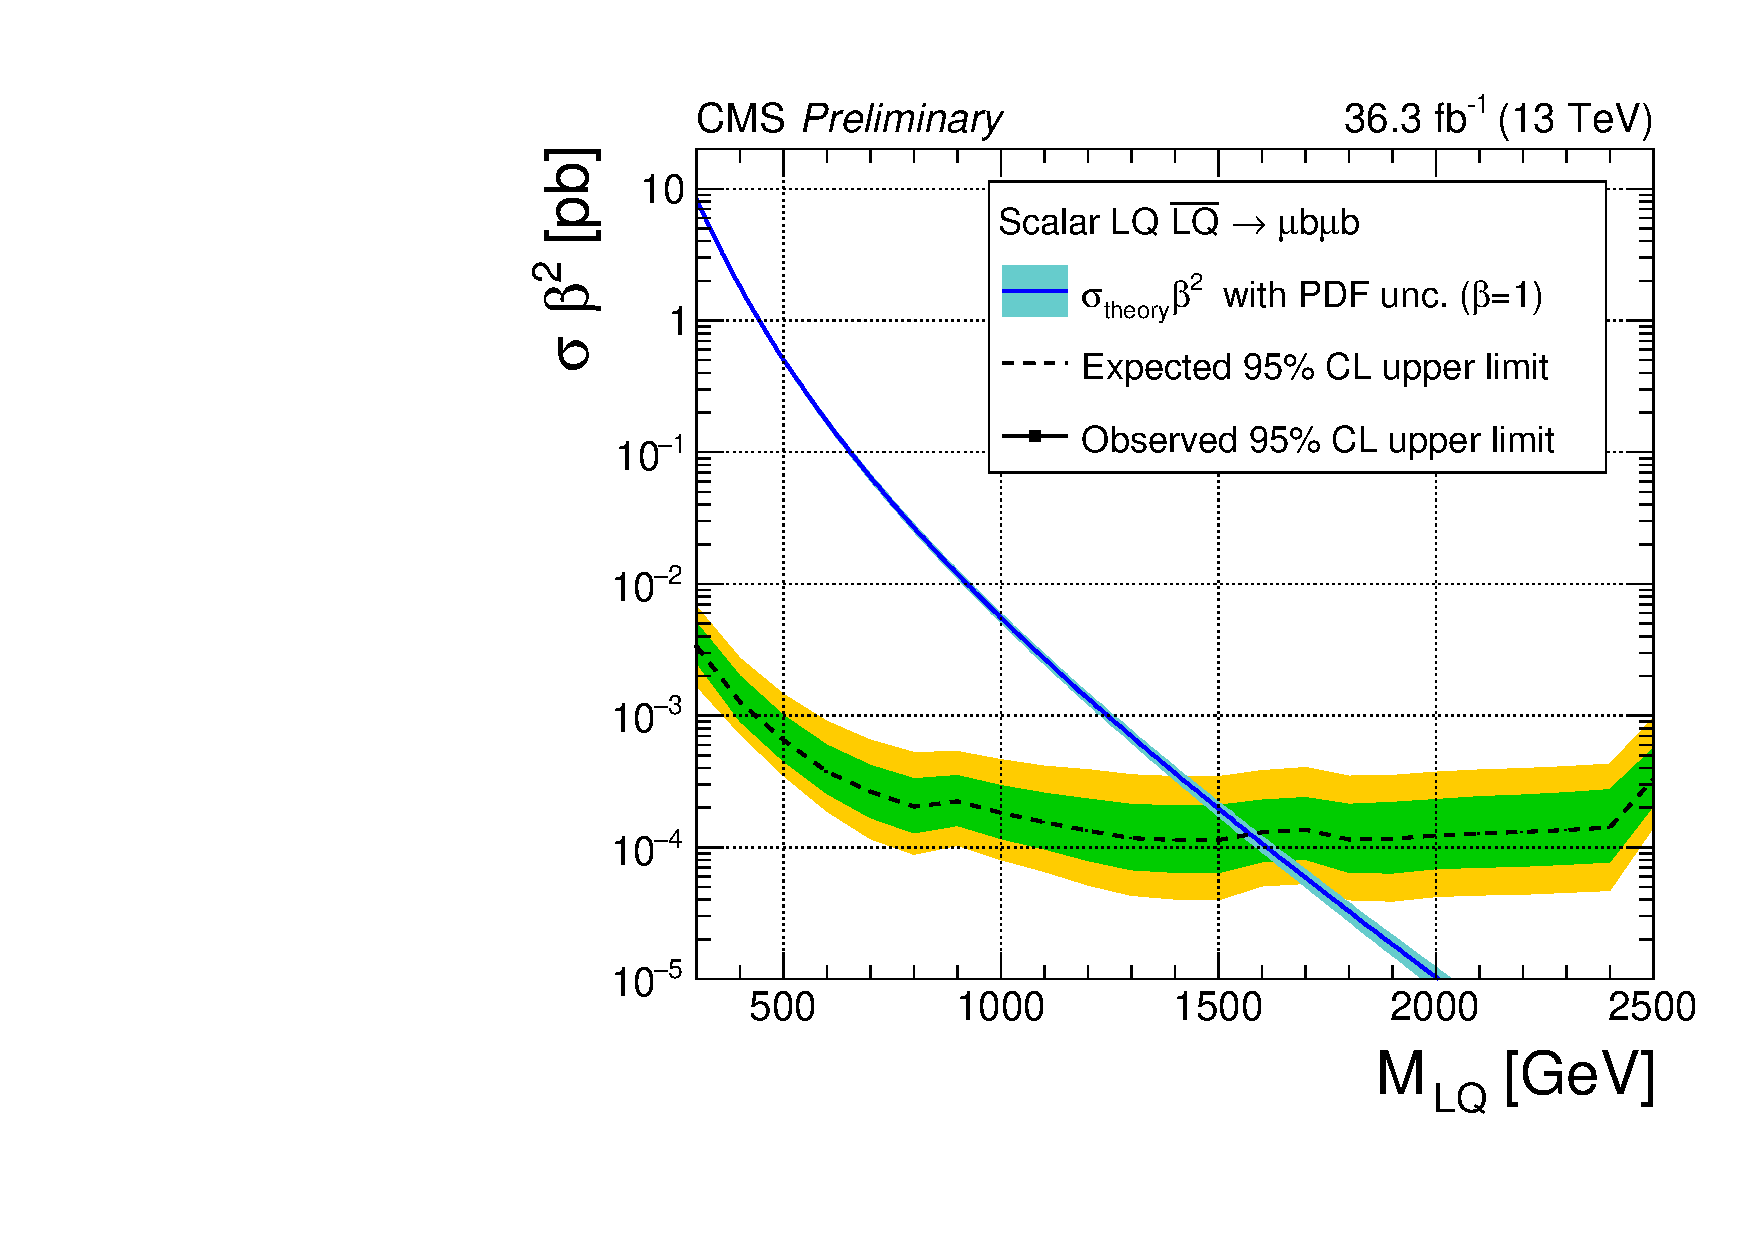
\includegraphics[width=.32\textwidth]{Images/Analysis/BDT_Study_plots/BR_Sigma_MuMu_2016_BDTStudy_Up.pdf}}
    {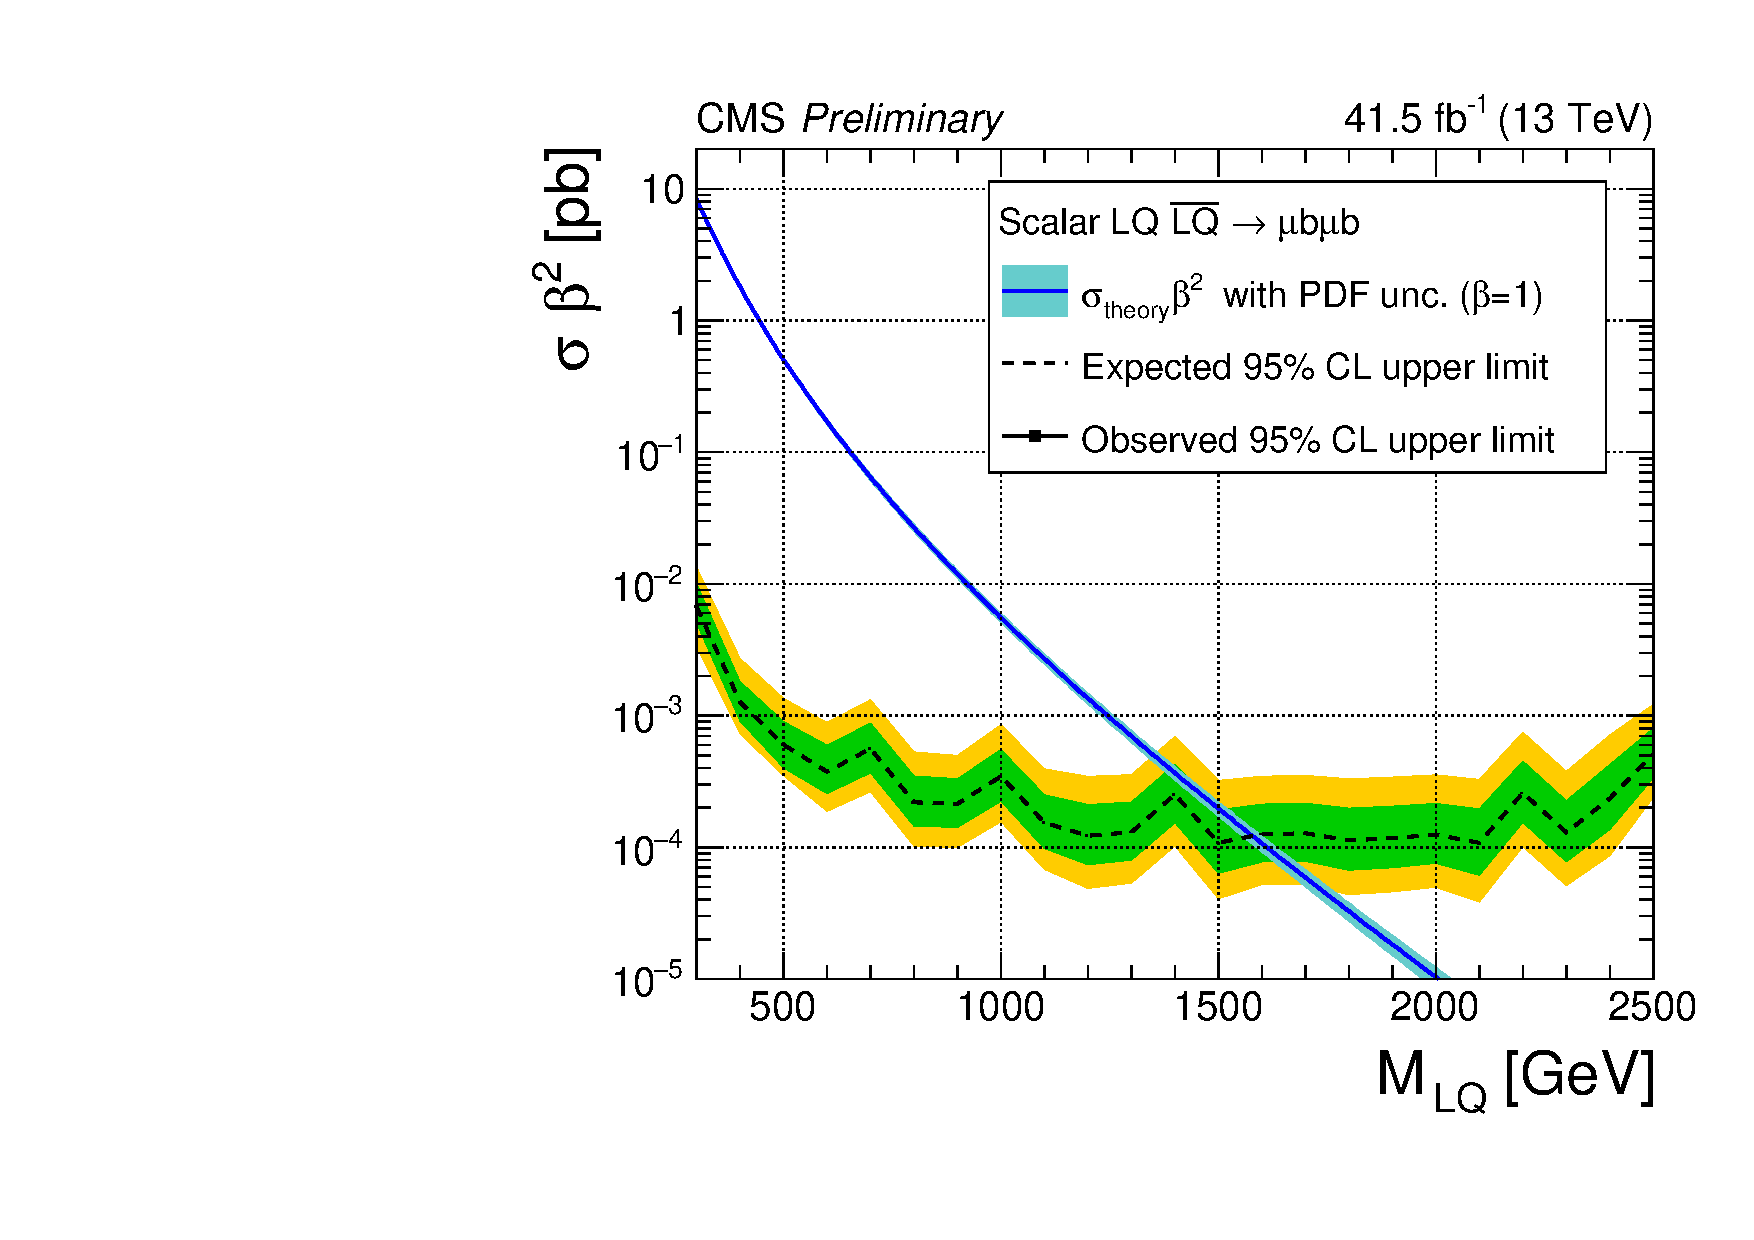
\includegraphics[width=.32\textwidth]{Images/Analysis/BDT_Study_plots/BR_Sigma_MuMu_2017_BDTStudy_Up.pdf}}
    {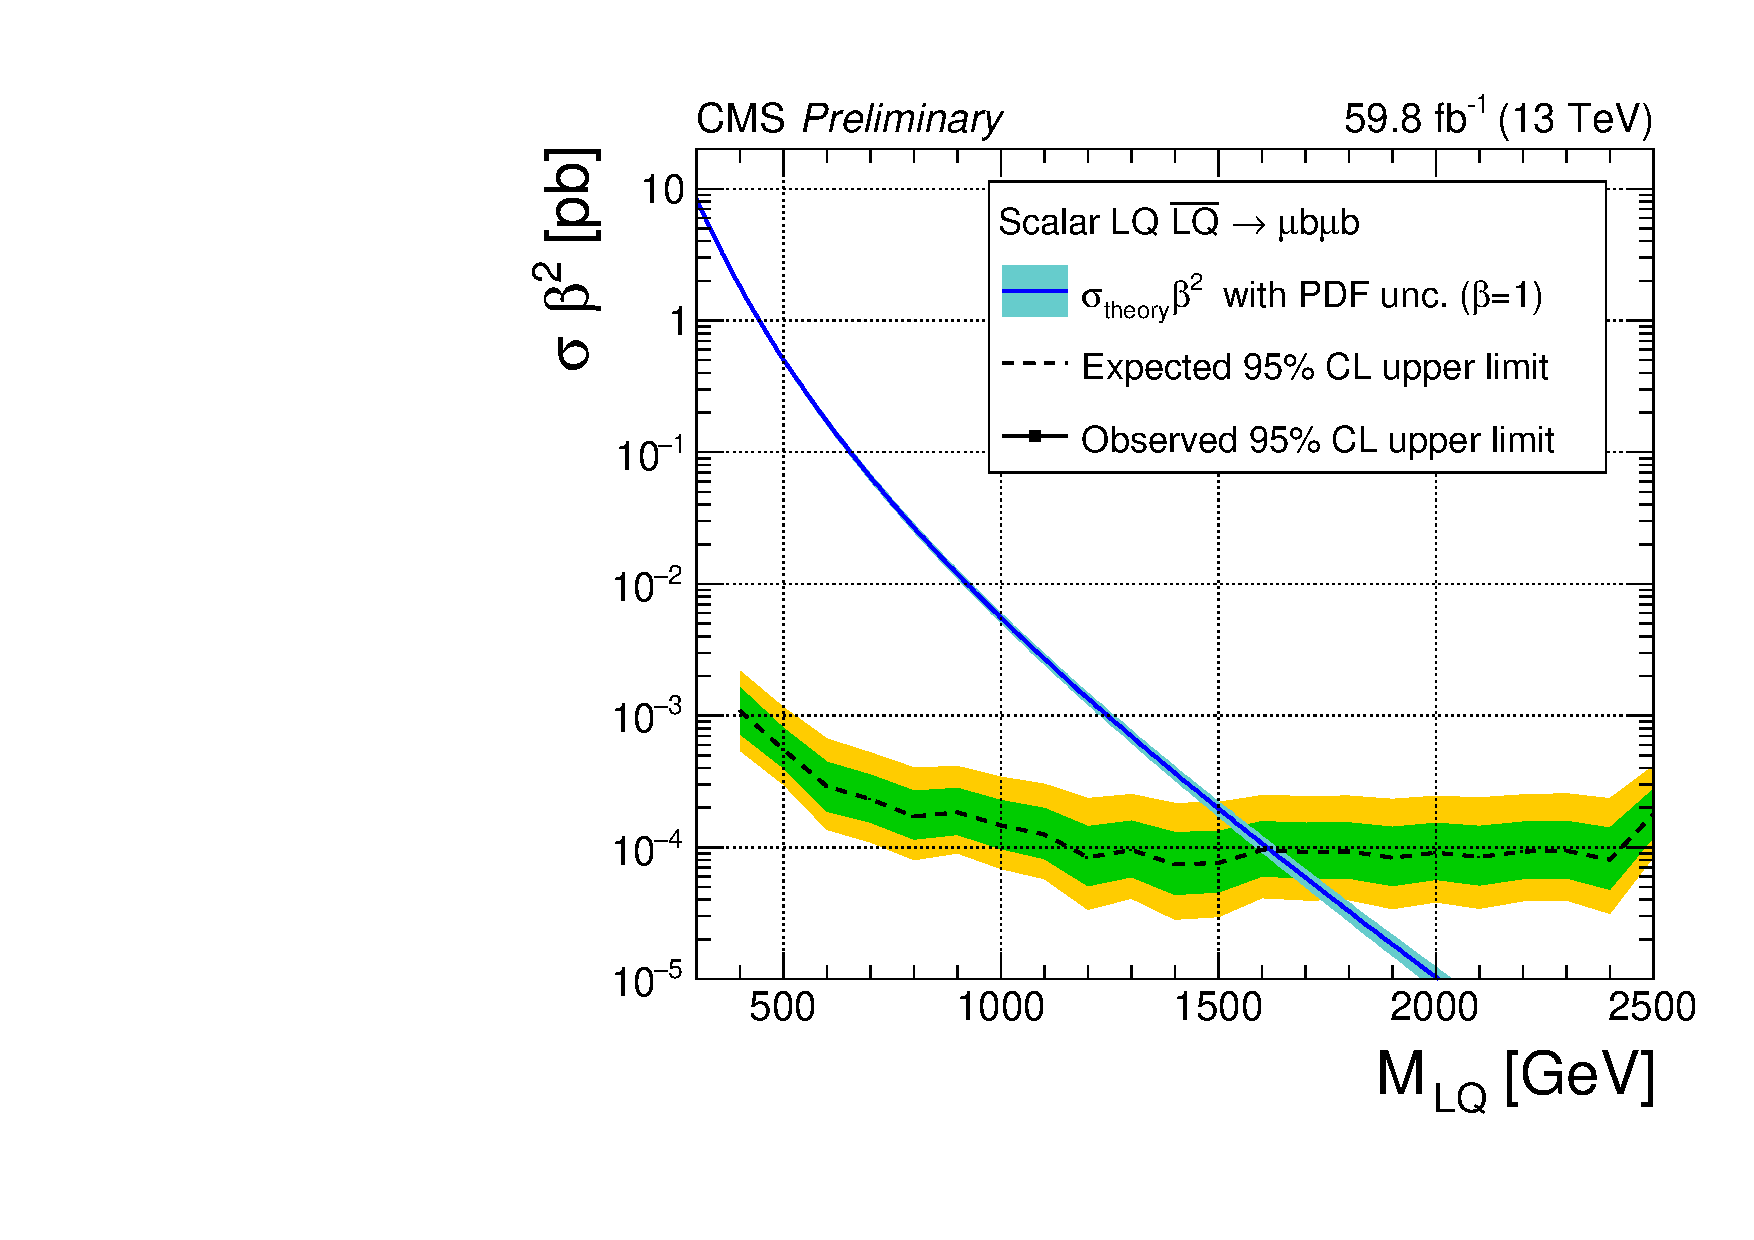
\includegraphics[width=.32\textwidth]{Images/Analysis/BDT_Study_plots/BR_Sigma_MuMu_2018_BDTStudy_Up.pdf}}
    \caption{The asymptotic expected upper limits at \SI{95}{\%} \CL placed on $\sigma\times\beta^2$ at each leptoquark mass hypothesis \MLQ. Limits set with a BDT trained on one mass point above (top) and one mass point below (bottom) the leptoquark mass hypothesis in 2016 (left), 2017 (middle), and 2018 (right) simulation.}
    \label{figapp:BDTstudy}
\end{figure}

\begin{figure}[htbp]
    \centering
    {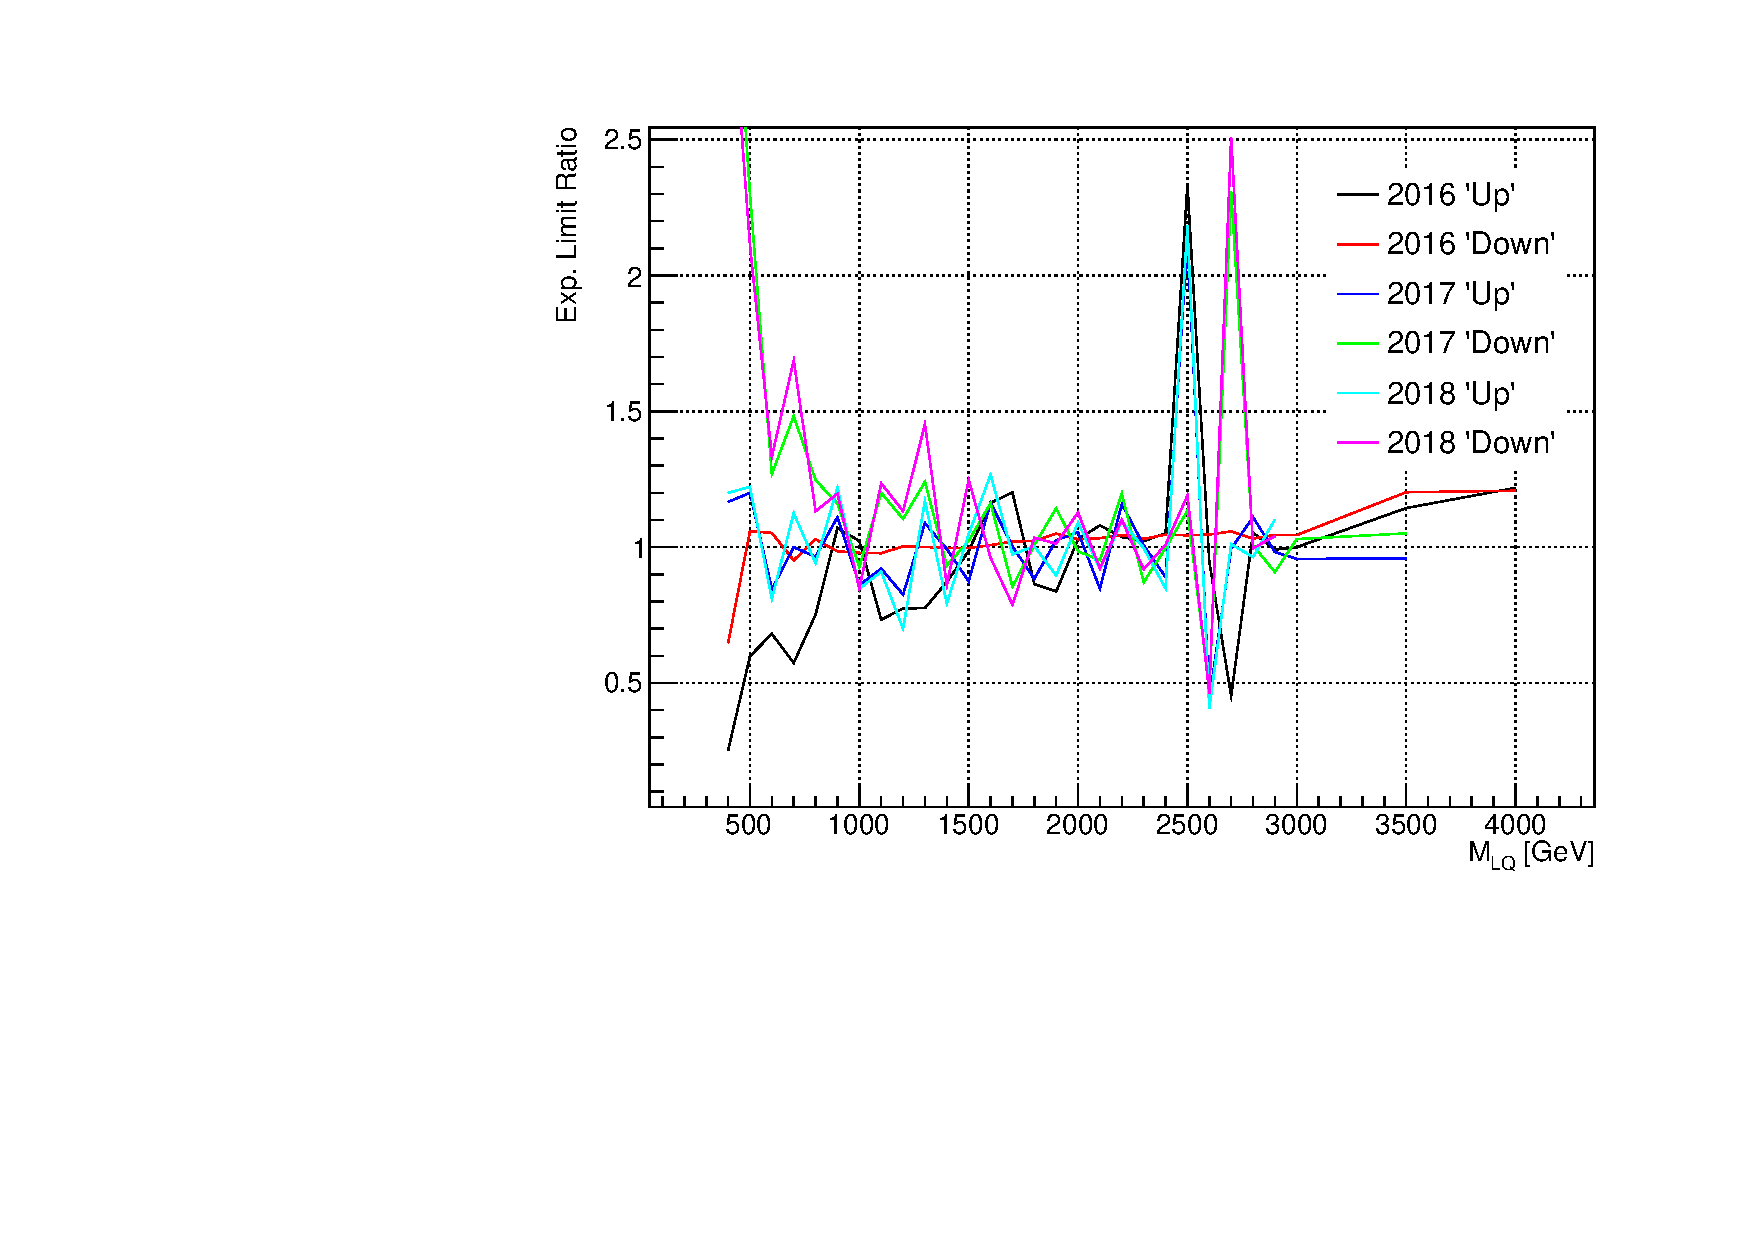
\includegraphics[width=.49\textwidth]{Images/Analysis/BDT_Study_plots/BDTStudyLimitRatio.pdf}}
    {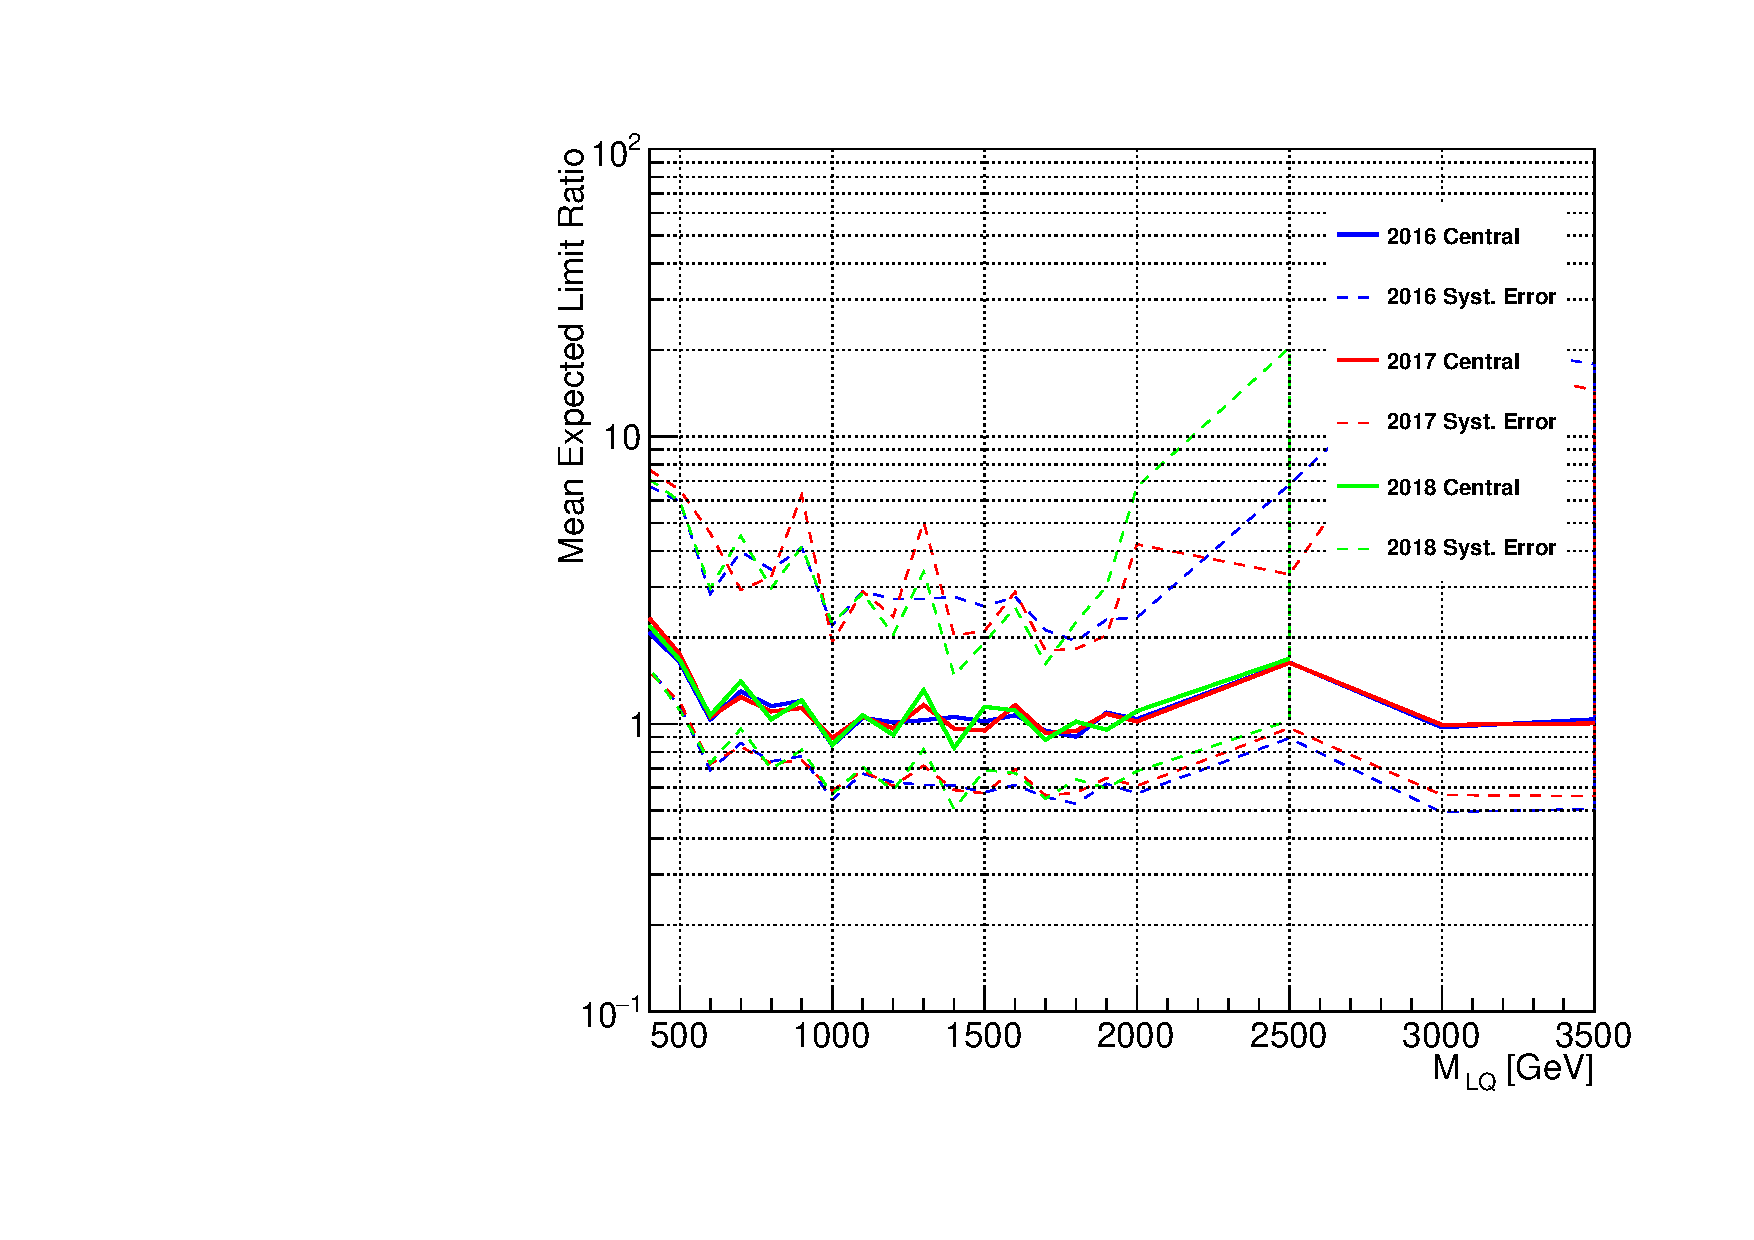
\includegraphics[width=.49\textwidth]{Images/Analysis/BDT_Study_plots/BDTStudyLimitAverageRatio2016_RmHighMass.pdf}}
    \caption{(Left) The ratios of the asymptotic expected upper limits placed on $\sigma\times\beta^2$ at each leptoquark mass hypothesis, where the numerator is the limit using the ``up'' or ``down'' varied BDT training mass point and the denominator is the limit using the nominal BDT training mass point (the same mass as the leptoquark mass hypothesis). (Right) The average of the ratios over the two variations (solid lines) with uncertainty bands (dashed lines) corresponding to $\pm 1$ standard deviations.}
    \label{figapp:BDTratio}
\end{figure}